\mychapter{Introdução}
\label{cap:introducao}

Segundo \citeasnoun{ribeiro:1999}, o termo automação está relacionado com a
substituição da mão-de-obra humana ou animal por uma máquina que realize uma
função equivalente. Partindo desse princípio, pode-se dizer que a automação
surge na sociedade em meados do século X, com os moinhos hidráulicos que
produziam farinha. Tal mecanismo, capaz de substituir o trabalho de dez a vinte
homens, levou a um crescimento da produção de alimentos nunca antes observado.

Desde então, o homem tem direcionado seu conhecimento para o desenvolvimento de
tecnologias que o auxiliem em suas atividades. Com a revolução industrial, a
partir da segunda metade do século XVIII, o processo de transformação e
desenvolvimento dessas tecnologias foi acelerado, de tal forma que o homem foi
capaz de produzir uma máquina a vapor para movimentar equipamentos industriais e
de fazer um martelo de 60 quilos dar 150 golpes por minuto \cite{goeking:2010}.

Por outro lado, a utilização de sistemas de controle remete a tempos ainda mais
antigos, por volta de 300 a.C. a 250 a.C., quando foram desenvolvidas as
primeiras bóias flutuadoras, o relógio de água de Ktsíbios e uma lamparina a
óleo que matinha o nível de óleo combustível constante
\cite{mayr:1970,mayr:1971,mayr:1975}.

Já na Europa Moderna, o primeiro sistema com realimentação a ser inventado foi o
regulador de temperatura de Cornelis Drebbel, entre o final do século XVI e
início do século XVII \cite{mayr:1975}. No final do século XVII e início do
século XVIII, Dennis Papin inventou o primeiro regulador de pressão para
caldeiras a vapor. Tal dispositivo tinha funcionalidade semelhante a uma válvula
de segurança de uma panela de pressão \cite{dorf:2009}. 

% ------------------------------------------------------------------------------
\section{Aspectos históricos do controle automático}
A junção dos conceitos acima discutidos se dá no final do século XVIII, quando,
em 1769, James Watt desenvolve o primeiro controlador automático com
realimentação usado em um processo industrial, conhecido como {\it regulador de
esferas}.

O dispositivo, inteiramente mecânico, mostrado na Fig.
\ref{fig:controlador_james}, controlava a velocidade de um motor a vapor através
do movimento de duas esferas. Na medida em que a velocidade do eixo de saída do
motor a vapor aumentava, as esferas eram elevadas (força centrífuga) e a válvula
era fechada, diminuindo o fluxo de vapor para o motor e, consequentemente, sua
velocidade. No caso oposto, quando a velocidade de saída do eixo do motor a
vapor reduzia, as esferas eram rebaixadas, abrindo a válvula e aumentando o
fluxo de vapor para o motor, o que, consequentemente, aumentava sua velocidade
\cite{mayr:1970,mayr:1975,dorf:2009}.

\begin{figure}[htb]
\centering
    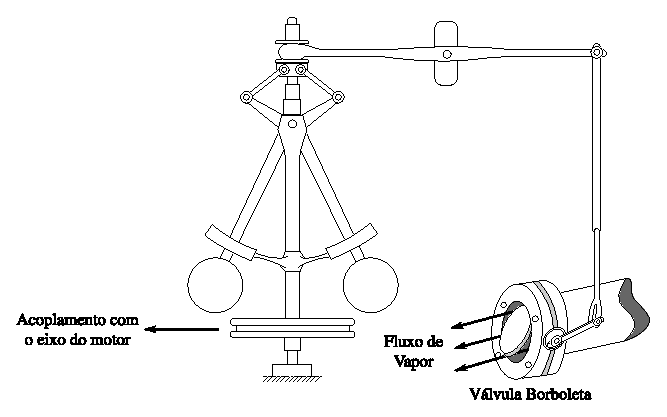
\includegraphics{imgs/introducao/eps/regulador_esferas}
    \caption{Regulador de Esferas de James Watt.}
    \label{fig:controlador_james}
\end{figure}

Ainda em 1769, segundo \citeasnoun{faccin:2004}, Richard Arkwright, um inventor
inglês considerado um dos precursores das técnicas de produção em série,
acelerou o processo de industrialização ao desenvolver uma máquina de tecer
movimentada pela força da água corrente. Segundo ele, foi o tear mecânico que
impulsionou a Revolução Industrial na Europa, contribuindo diretamente para a
mudança dos hábitos de trabalho e das relações sociais da Idade Contemporânea. 

De acordo com \citeasnoun{dorf:2009}, o século seguinte foi caracterizado pelo
desenvolvimento de sistemas de controle automático através da intuição e da
invenção. Esforços para aumentar a exatidão dos sistemas de controle levaram a
atenuações mais lentas das oscilações transitórias e até mesmo a sistemas
instáveis, tornando-se necessário o desenvolvimento da teoria de controle
automático.

Por volta de 1868, J. C. Maxwell formulou a teoria matemática, através das
equações diferenciais do regulador de esferas de James Watt, relacionando os
efeitos dos parâmetros do sistema com o seu desempenho \cite{maxwell:1964}. Com
o seu trabalho, Maxwell demonstrou a importância e a utilidade de modelos e
métodos matemáticos para a compreensão dos processos industriais e da teoria de
controle.

Nos anos seguintes, E. J. Routh (1877) e A. Hourwitz (1885) criaram seus
critérios de estabilidade de maneira independente
\cite{routh:1877,bennett:1996,faccin:2004}.

% ------------------------------------------------------------------------------
\section{Importância da automação}

% ------------------------------------------------------------------------------
\section{Falhas}

% ------------------------------------------------------------------------------
\subsection{Tipos de falhas}

% ------------------------------------------------------------------------------
\subsection{Detecção}

% ------------------------------------------------------------------------------
\subsection{Métodos de detecção}

% ------------------------------------------------------------------------------
\subsection{Detecção de falhas com RNAs}
